\scanpage{130}

\diagram{\begin{tikzcd}[ampersand replacement=\&,column sep=small]
\unsure{B|A}\arrow[dr,dash]\&\& B'\arrow[dl,dash]\\
\&A\&
\end{tikzcd}}

\diagram{\begin{tikzcd}[ampersand replacement=\&,column sep=small]
\&\&X\times_S\!X\arrow[dl,dash]\arrow[dr,dash]\&\&\\
G\&X\arrow[dr,dash]\&\&X'\arrow[dl,dash]\&G'\\
\&\&s,s'\in S\&\&
\end{tikzcd}}

$X$ tot. ramifié en $s$, étale en dehors

$X'$ tot. ramifié en $s'$, étale en dehors

$X,X'$ normaux irréd.

$X\times_S X'$ est \unsure{norm.|normal|connexe} ?

\diagram{\begin{tikzcd}[ampersand replacement=\&,column sep=small]
\&\pi_1(S-\{s,s'\})\arrow[dl,dash]\arrow[dr]\&\\
\pi_1(S-s)\arrow[dr]\&\&\pi_1(S-s')\arrow[dl]\\
\&\pi_1(S)\&
\end{tikzcd}}

\diagram{\begin{tikzcd}[ampersand replacement=\&,column sep=small]
\&G*\mathbb Z*\mathbb Z\arrow[dl]\arrow[dr]\&\&G\times G'\\
X*\mathbb Z\arrow[dr]\&\&G*\mathbb Z\arrow[dl]\&\\
\&G\&\&
\end{tikzcd}}

\diagram{\begin{tikzcd}[ampersand replacement=\&,column sep=small]
\&\deleted{\unsure{X}}\arrow[dl,dash]\arrow[dr,dash]\&\\
\deleted{X_s}\arrow[dr]\&\&\deleted{X'_s}\arrow[dl]\\
\&S\&
\end{tikzcd}}

\figure{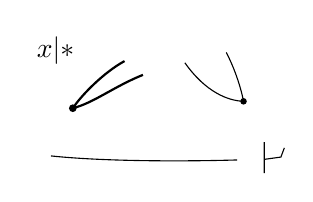
\begin{tikzpicture}[x=.73cm,y=.73cm]
\node at (-.2,1.20) {$\deleted{\unsure{x|\ast}}$};
\draw[thick] (1.00,1.02).. controls (.65,.83) and (.26,.44)..(.10,.20)..controls (.46,.29) and (.82,.58)..(1.32,.78);
\fill (.10,.20) circle (.067);
\draw (2.05,.99)..controls (2.41,.48) and (2.8,.33)..(3.07,.32)..controls (3.02,.58) and (2.91,.90)..(2.77,1.17);
\fill (3.07,.32) circle (.057);
\draw (-.28,-.63)..controls (.77,-.74) and (2.3,-.72)..(2.96,-.70) (3.43,-.39)--(3.43,-.93) (3.43,-.69)--(3.72,-.65)--(3.78,-.49);
\end{tikzpicture}}

\diagram{\begin{tikzcd}[ampersand replacement=\&,column sep=small]
\&I\subset H_s\subset G\times G'\arrow[dl,"\text{surj}"']\arrow[dr,"\text{surj}"]\&\\
G\&\&G'
\end{tikzcd}}

\diagram{\begin{tikzcd}[ampersand replacement=\&,column sep=large,row sep=large]
\&Z\subset X\times_S X\arrow[dl, "{\substack{\text{\unsure{comp. irr.|comp. revêt.}}\\ \text{tot. ramifié}\\\text{en les pts de }X_{s'}}}"']\arrow[dr,"{\text{tot. ram. en les pts de }X'_s}"]\&\\
X\&\&X'
\end{tikzcd}}

\[
\vdots\qquad(\mathbb Z/4\mathbb Z)^*\ \text{d'ordre }2\qquad\mathbb Z/
\]

% archive sheet number: 129
